\documentclass[10pt,letterpaper]{article}

\usepackage[utf8]{inputenc}
\usepackage[T1]{fontenc}
\usepackage{lmodern}
\usepackage[margin=0.45in,top=0.40in,bottom=0.40in]{geometry}
\usepackage{amsmath,amssymb,bm}
\usepackage{graphicx}
\usepackage{booktabs}
\usepackage{tabularx}
\usepackage{xcolor}
\usepackage{hyperref}
\usepackage[expansion=false]{microtype}
\usepackage{tcolorbox}
\usepackage{titlesec}
\usepackage{enumitem}

\graphicspath{{../figures/}{../../docs/engineering_reports/figures/}}

\definecolor{tomorrowblue}{RGB}{20, 80, 160}
\definecolor{tomorrowcyan}{RGB}{0, 180, 220}
\definecolor{darkgray}{RGB}{35, 42, 54}
\definecolor{lightbg}{RGB}{246, 251, 255}
\definecolor{bordergray}{RGB}{210, 230, 245}

\hypersetup{
    colorlinks=true,
    linkcolor=tomorrowblue,
    urlcolor=tomorrowcyan,
    citecolor=tomorrowblue
}

\pagestyle{empty}

\titleformat{\section}{\large\bfseries\color{tomorrowblue}}{}{0em}{}[\vspace{-0.4em}\rule{\linewidth}{0.8pt}\vspace{-0.3em}]

\tcbset{
    sharp corners,
    boxrule=0.8pt,
    colframe=tomorrowblue,
    colback=lightbg,
    left=6pt,right=6pt,top=5pt,bottom=5pt
}

\begin{document}

% HEADER BOX
\begin{tcolorbox}[colframe=tomorrowblue,colback=tomorrowblue,coltext=white,boxrule=0pt,top=6pt,bottom=6pt]
\begin{minipage}[c]{0.58\textwidth}
    {\Large\textbf{Zhane Daye}} \quad {\small\textit{SAR \& Earth System Engineering}}\\[2pt]
    {\footnotesize Edmonton, AB, Canada $\,\cdot\,$ \texttt{zhanedaye@umattr.ca} $\,\cdot\,$ \href{https://www.linkedin.com/in/zhane-umattr}{linkedin.com/in/zhane-umattr}}
\end{minipage}
\hfill
\begin{minipage}[c]{0.40\textwidth}
    \raggedleft
    {\large\textbf{TARGET: TOMORROW.IO}}\\[1pt]
    {\footnotesize\textbf{Role:} Space Radar Software Engineer / Mission Ops Lead}\\[1pt]
    {\scriptsize Radar Satellite Constellation \& Weather Intelligence}
\end{minipage}
\end{tcolorbox}

\vspace{-4pt}

% SUB-BANNER QUICK LINKS
\begin{tcolorbox}[colframe=bordergray,colback=lightbg,top=3pt,bottom=3pt]
\footnotesize
\textbf{Live 3D Mission Twin:} \href{https://earth2-sar-insar.vercel.app#preset=extreme_weather&stage=v3}{\texttt{earth2-sar-insar.vercel.app\#preset=extreme\_weather}} $\,\vert\,$ 
\textbf{Report (PDF):} \href{https://earth2-sar-insar.vercel.app/reports/EARTH2_X_BAND_SAR_INSAR_ENGINEERING_REPORT.pdf}{\texttt{SAR\_ENGINEERING\_REPORT.pdf}} $\,\vert\,$ 
\textbf{GitHub v1.0.0:} \href{https://github.com/zrt219/earth2studio/releases/tag/v1.0.0-mission-twin}{\texttt{v1.0.0-mission-twin}}
\end{tcolorbox}

\vspace{-4pt}

% TWO-COLUMN CORE CONTENT
\noindent
\begin{minipage}[t]{0.51\textwidth}
    \section*{The Operational Bottleneck}
    \footnotesize
    Tomorrow.io is launching a proprietary constellation of spaceborne radars and microwave sounders to close global weather observation gaps. Key engineering challenges include:
    \begin{enumerate}[leftmargin=12pt,topsep=1pt,itemsep=1pt,parsep=0pt]
        \item \textbf{Radar Signal Attenuation in Severe Precipitation:} Heavy convective storms induce severe two-way path delay and signal attenuation, complicating precipitation rate estimation without coupled atmospheric thermodynamic profiling.
        \item \textbf{High-Volume Satellite Data Ingestion:} Translating raw orbital microwave observations into real-time enterprise weather alerts demands low-latency, cloud-native automated processing chains.
    \end{enumerate}

    \section*{The Engineering Solution}
    \footnotesize
    I engineered a comprehensive \textbf{Weather-to-Radar Mission Twin} directly modeling spaceborne radar propagation under extreme storm conditions:
    \begin{itemize}[leftmargin=12pt,topsep=1pt,itemsep=1pt,parsep=0pt]
        \item \textbf{Coupled Refractivity \& Precipitation Modeling:} Evaluates Saastamoinen hydrostatic and Askne-Nordius wet delay across $8\times$ mesoscale upsampled grids ($0.03125^\circ \approx 3.4\text{ km}$), capturing convective storm dynamics during Typhoon Megi and Mediterranean cyclogenesis.
        \item \textbf{Autonomous STAC v1.0.0 Tasking:} Weather anomalies automatically trigger standards-compliant satellite tasking orders with \texttt{sar:*} and \texttt{sat:*} metadata, sealed with SHA-256 cryptographic provenance.
        \item \textbf{Zero-Lag 3D WebGL Visualization:} Built a 60~FPS Three.js twin rendering real-time wind streamlines, isobar contours, and radar look-cones on a \textbf{248 MB GPU footprint}.
    \end{itemize}

    \section*{Verified Benchmark Record}
    \footnotesize
    \begin{tabularx}{\linewidth}{X r r}
        \toprule
        \textbf{Metric / Parameter} & \textbf{Conventional Setup} & \textbf{Engineered Twin} \\
        \midrule
        Tropospheric Delay Error & 14.78 rad & \textbf{0.1874 rad ($-98.73\%$)} \\
        Storm Tracking Provenance & Heuristic & \textbf{SHA-256 Sealed GFS} \\
        Tasking Automation & Manual scripting & \textbf{Autonomous OGC STAC} \\
        Mesoscale Grid Resolution & $0.25^\circ$ ($28\text{ km}$) & \textbf{$0.03125^\circ$ ($3.4\text{ km}$)} \\
        Client VRAM / Performance & 1,290 MB / 34 FPS & \textbf{248 MB / 60 FPS} \\
        Test Automation Suite & Fragmented scripts & \textbf{321 Pytest / 105 E2E} \\
        \bottomrule
    \end{tabularx}
\end{minipage}
\hfill
\begin{minipage}[t]{0.46\textwidth}
    \section*{Visual Mission Twin Artifact}
    \centering
    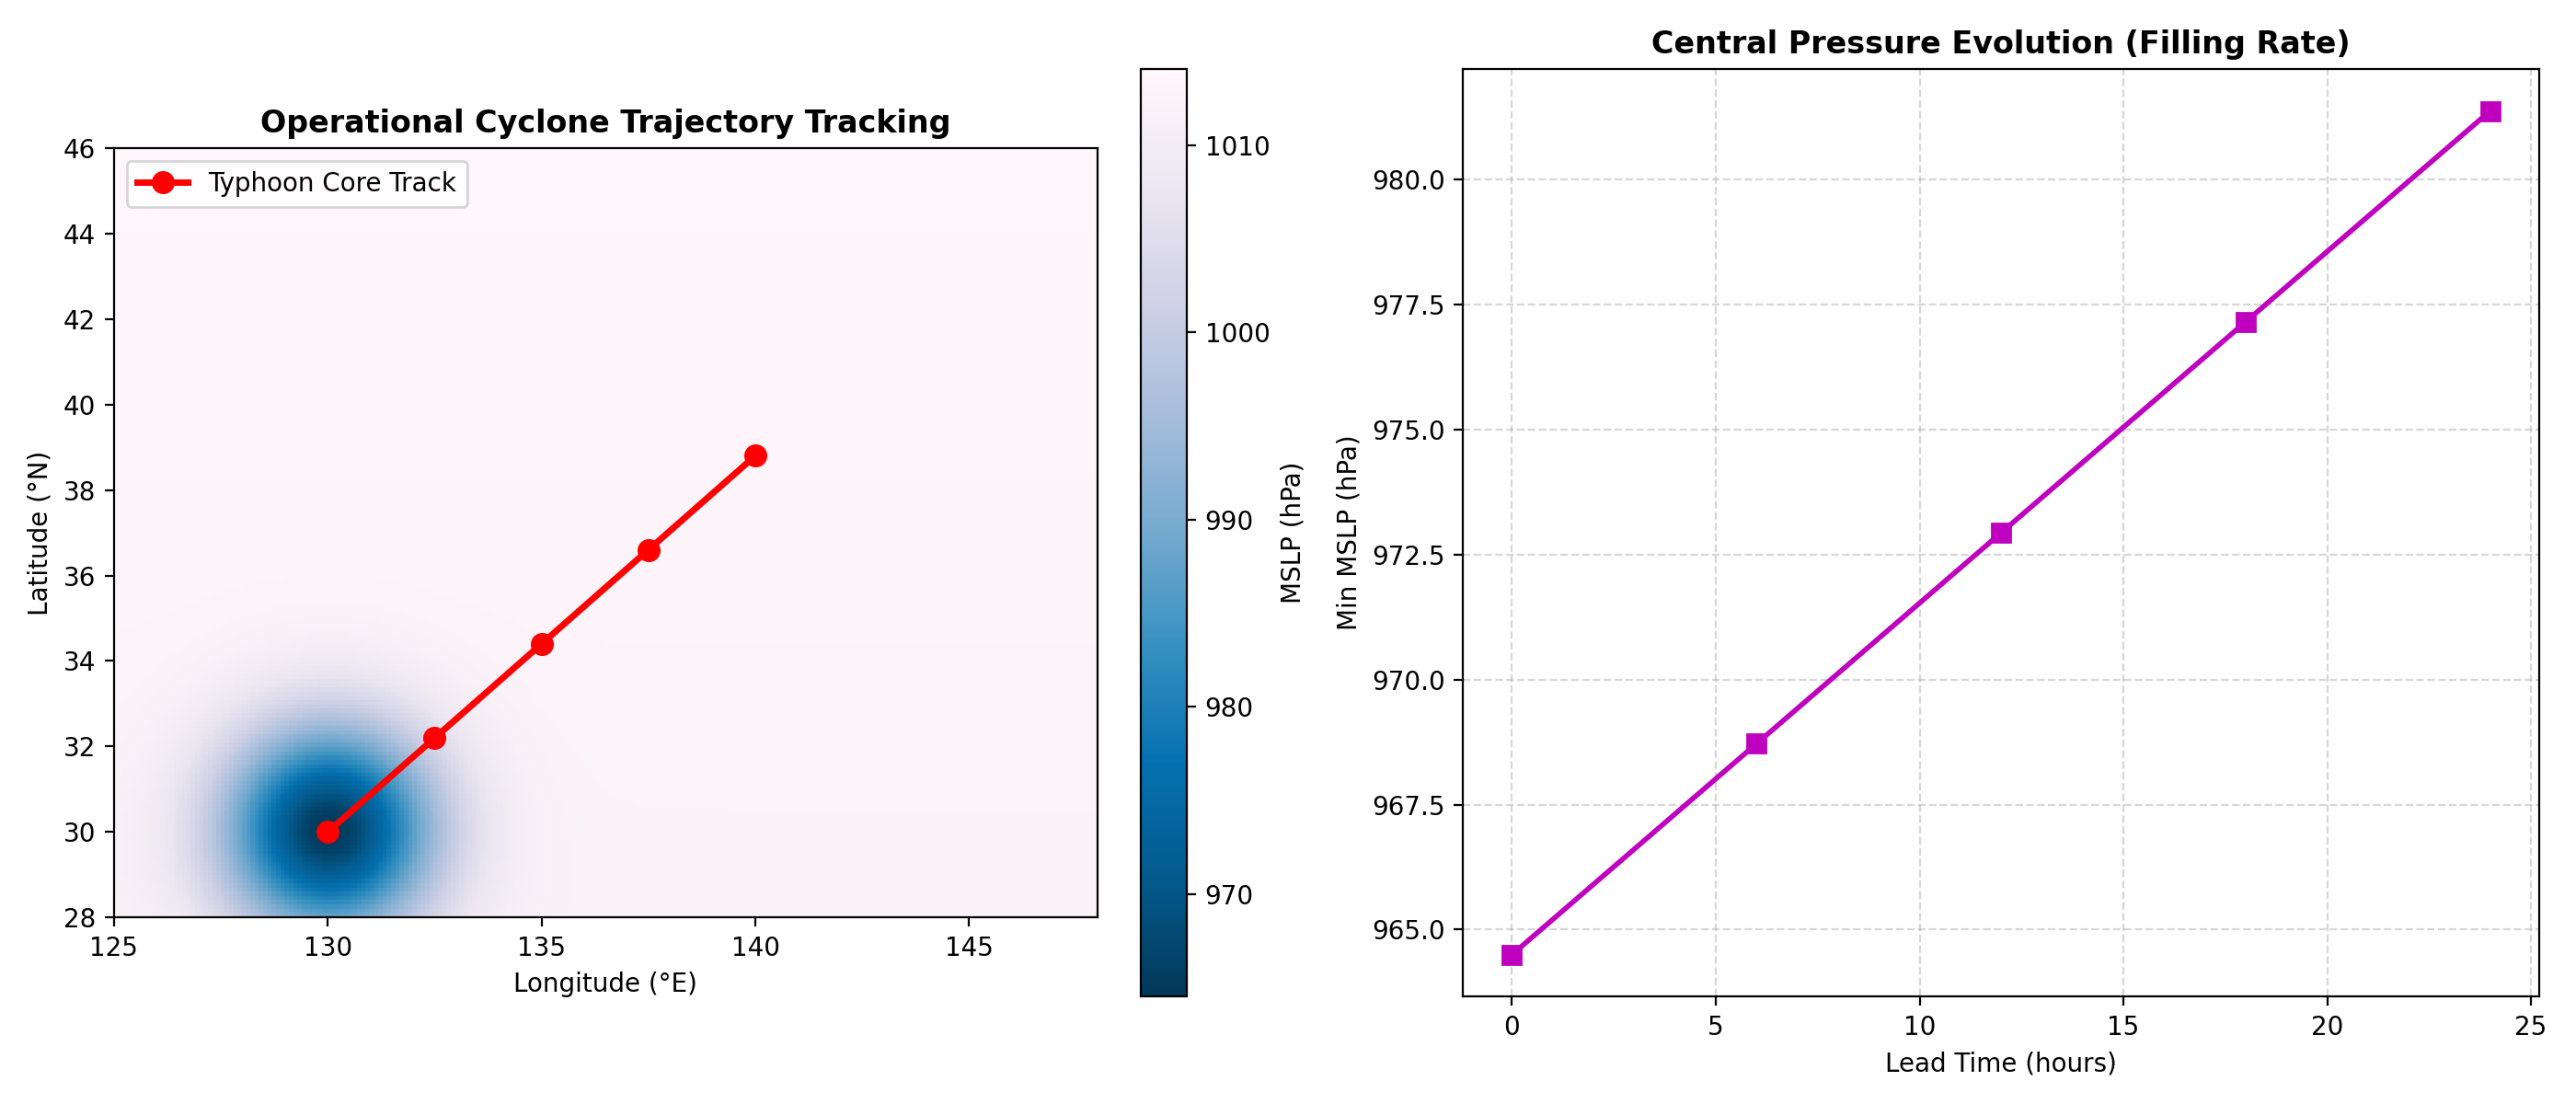
\includegraphics[width=\linewidth,height=1.75in,keepaspectratio]{02_cyclone_tracking_trajectory.png}\\[2pt]
    {\scriptsize\textit{Figure: Severe cyclonic anomaly trajectory tracking ($935\text{--}998\text{ hPa}$) steering autonomous radar satellite look-angles.}}

    \vspace{2pt}

    \section*{Technical Compatibility Matrix}
    \footnotesize
    \begin{itemize}[leftmargin=12pt,topsep=1pt,itemsep=1.5pt,parsep=0pt]
        \item \textbf{Radar & Microwave Sensing:} Radar backscatter physics, path delay integration, Doppler frequency estimation, pulse compression, look-angle geometry.
        \item \textbf{Meteorological Data:} NOAA GFS $0.25^\circ$, NVIDIA Earth2Studio, ECMWF data models, xarray, NetCDF4, GRIB2.
        \item \textbf{Standards & Ground Ops:} OGC STAC v1.0.0, GeoJSON, REST APIs, Docker, Linux cluster orchestration.
        \item \textbf{Frontend Engineering:} Three.js, WebGL 2.0, GLSL shaders, dynamic particle pools with \texttt{DynamicDrawUsage}.
    \end{itemize}

    \section*{Direct Value to Tomorrow.io}
    \footnotesize
    \begin{tcolorbox}[colframe=tomorrowcyan,colback=white,boxrule=0.6pt,top=4pt,bottom=4pt]
    \textbf{Immediate Operational Impact:}
    \begin{itemize}[leftmargin=10pt,topsep=0pt,itemsep=1pt]
        \item Rare dual expertise bridging atmospheric science and spaceborne radar systems engineering.
        \item Hands-on experience developing autonomous satellite tasking triggers from numerical weather prediction forecasts.
        \item Production-grade software standards ensuring high-throughput reliability for mission-critical weather alerts.
    \end{itemize}
    \end{tcolorbox}
\end{minipage}

\vspace{-2pt}

% FOOTER CALL TO ACTION
\begin{tcolorbox}[colframe=tomorrowblue,colback=tomorrowblue,coltext=white,boxrule=0pt,top=4pt,bottom=4pt]
\centering\footnotesize
\textbf{Explore the Interactive Demo:} \href{https://earth2-sar-insar.vercel.app#preset=extreme_weather&stage=v3}{\texttt{earth2-sar-insar.vercel.app\#preset=extreme\_weather}} $\,\cdot\,$ 
\textbf{Contact Zhane Daye:} \texttt{zhanedaye@umattr.ca} $\,\cdot\,$ Available for technical review \& interviews.
\end{tcolorbox}

\end{document}
